\documentclass[11pt, twoside, a4paper]{book}

\usepackage{graphicx}
\usepackage[utf8]{inputenc}
\usepackage{ngerman}
%\usepackage{lineno}
\usepackage{verbatim}
\usepackage[squaren]{SIunits}
\usepackage{amsmath}
\usepackage{amsfonts}
\usepackage{amssymb}
\usepackage{enumitem}
\usepackage{fancyhdr}
\usepackage{textcomp}
\usepackage{subcaption}
\usepackage[noadjust]{marginnote}
\usepackage{tikz}
\usepackage{nicefrac}
\usepackage{framed}
\usepackage{import}

\usetikzlibrary{calc,intersections}
\usetikzlibrary{arrows}
\usetikzlibrary{decorations.markings}
\usetikzlibrary{decorations.pathreplacing}
\usepackage[european resistors]{circuitikz}
\usepackage[ 
    top=2cm, 
    bottom=2cm, 
    outer=3cm, 
    inner=3cm,
    marginparwidth=2.5cm,
		headheight=14pt
  ]{geometry}

\usepackage{parskip}
\usepackage{pdfpages}

\setlength{\parindent}{0pt}

\newcommand{\experimentheader}[4]
{
  \iftutor{{\bf Schwierigkeitsgrad:} #1\\}
  \iftutor{{\bf Dauer:} #2\\}
  {\bf Ger\"ate:} #3\\
  {\bf Bauteile:} #4
}

\newcommand{\hintboxNone}{0}
\newcommand{\hintboxExclamation}{1}
\newenvironment{hintbox}[4][\hsize]
{
  \def\FrameCommand
  {%
    {\color{#3}\vrule width 3pt}%
    \hspace{0pt}%must no space.
    \fboxsep=\FrameSep\colorbox{#4}%
  }%
  \MakeFramed{\hsize#1\advance\hsize-\width\FrameRestore}%
  \mbox{\textbf{#2}:}%
}
{
  \endMakeFramed
}
\newcommand{\xhintbox}[3]
{
  \begin{hintbox}{Achtung}{red!50}{red!10}
    #3
  \end{hintbox}
}

\newenvironment{hint}
{
  \begin{hintbox}{Hinweis}{green!50}{green!10}
}
{
  \end{hintbox}
}

\newenvironment{definition}
{
  \begin{hintbox}{Definition\\}{white!50}{white!10}
}
{
  \end{hintbox}
}

\newenvironment{important}
{
  \begin{hintbox}{Hinweis}{gray!50}{gray!10}
}
{
  \end{hintbox}
}

\newenvironment{jason}
{
  \begin{hintbox}{Achtung}{red!50}{red!10}
}
{
  \end{hintbox}
}

\newcommand{\mandatoryenumi}
{
  \renewcommand{\labelenumi}{\arabic{enumi}.} 
}
\newcommand{\optionalenumi}
{
  \renewcommand{\labelenumi}{$\bigstar$\quad\arabic{enumi}.} 
}
\newcommand{\mandatoryenumii}
{
  \renewcommand{\labelenumii}{(\alph{enumii})} 
}
\newcommand{\optionalenumii}
{
  \renewcommand{\labelenumii}{$\bigstar$\quad(\alph{enumii})} 
}
\newcommand{\icname}[1]{\mbox{\tt #1}}


  %\newcommand{\iftutor}[1]{}
\newcommand{\ifnotutor}[1]{#1}

  \newcommand{\iftutor}[1]{#1}
\newcommand{\ifnotutor}[1]{}


\newenvironment{tutorhint}{\comment}{\endcomment}
\newenvironment{todo}{\comment}{\endcomment}
\newenvironment{solution}{\comment}{\endcomment}
\iftutor
{
  \renewenvironment{todo}
  {
    \hintbox{Todo}{red!50!yellow!90}{red!50!yellow!20}
  }
  {
    \endhintbox
  }
  \renewenvironment{tutorhint}
  {
    \hintbox{Tutorenhinweis der Stunde}{blue!50}{blue!10}
  }
  {
    \endhintbox
  }
  \renewenvironment{solution}
  {
    \hintbox{L\"osung}{black!80}{black!5}
  }
  {
    \endhintbox
  }
}
\newcommand{\etutorhint}[1]
{
  \iftutor{
    \tutorhint
      #1
    \endtutorhint
  }
}
\newcommand{\esolution}[1]
{
  \iftutor
  {
    \solution
    #1
    \endsolution
  }
}
\newcommand{\etodo}[1]
{
  \iftutor
  {
    \todo
    #1
    \endtodo
  }
}



\begin{document}

\renewcommand{\thechapter}{\arabic{chapter}}
\setcounter{chapter}{13}
\def\chaptername{Versuch}

\chapter{Ultraschall}
\label{vn:2}

\etodo{\textbf{Praktikumsleitung:} Vor Versuchsbeginn einen Eimer mit crushed Eis aus dem Lager zur Verfügung stellen. Sicher stellen, dass genügend Kochsalz vorhanden ist (für ein ganzes Semester reichen 12-15 Pakete.}

In diesem Versuch werden Eigenschaften der Ausbreitung von Wellen in Medien anhand einiger Anwendungen von Ultraschall untersucht.
%
%------------------------------------------------
\section{Stichworte}
%------------------------------------------------
Ultraschall, Ausbreitung von Wellen, Longitudinal- und Transversalwellen, Reflexion und Transmission, Beugung, Totalreflexion.
%
%------------------------------------------------
\section{Literatur}
%------------------------------------------------
Gehrtsen, Kapitel 3.4, 4.2.1-3; Demtröder, Kapitel 11.9
%
%------------------------------------------------
\section{Anwendungsbeispiele}
%------------------------------------------------
%
Elastische Wellen mit Frequenzen oberhalb der menschlichen Hörschwelle (15 bis 20~kHz) bis etwa 10~GHz nennt man \textit{Ultraschall}. Bei großen Frequenzen liegen die Wellenlängen im selben Bereich wie die von sichtbaren Licht, weshalb Beugungserscheinungen, die die Ausbreitung des hörbaren Schalls so komplizieren, an Bedeutung verlieren. Das Schallfeld kann sehr gut fokussiert werden und kann so zur Ortung und Hinderniserkennung durch Richtstrahlreflexion genutzt werden (z. Bsp. Sonar in der Schifffahrt, bei Fledermäusen und Delphinen). \\
In Materialien mit einfachem Molekülaufbau, z. Bsp. in Metallen ist die Absorption von Ultraschall sehr gering. Daher und wegen seiner Ungefährlichkeit im Vergleich mit anderen Strahlungsarten (Röntgen, hartes UV-Licht, Neutronen), wird Ultraschall in vielen Bereichen benutzt: Ultraschallechografie in Medizin, Werkstoffprüfung, Dickenmessung, externe Messung des Füllstandes von Tanks, Konzentrationsmessung in Lösungen. Die Untersuchung der Ausbreitung von longitudinalen und transversalen Erdbebenwellen erlaubt detaillierte Untersuchungen der Erdkruste, erbrachte die ersten Hinweise auf die flüssige Natur des Erdmantels und erlaubt die Triangulation der Epizentren von Erdbeben.
%
%------------------------------------------------
\section{Theoretischer Hintergrund}
%------------------------------------------------

\subsection{Deformation von Festkörpern}

Das Verhalten von Festkörpern unter Deformation ist recht kompliziert und mathematisch sehr anspruchsvoll. Da wir allerdings einige der Zusammenhänge brauchen, um die Ausbreitung von Wellen in Fluiden und Festkörpern zu verstehen, seien sie hier knapp zusammengefasst.

\subsubsection{Dehnung und Kompression}

Eine Kraft $F$, die an einem Draht mit der Querschnittsfläche $A$ zieht, verlängert diesen um ein Stück $\Delta l$. Bei nicht zu großer Kraft $F$ ist diese Verlängerung proportional zu $F$, zur Drahtlänge $l$ und zu $1/A$. Betrachten wir die relative Längenänderung $\epsilon = \Delta l/l$, so ergibt sich dieses \textit{Hooke'sche Gesetz}:
\begin{equation}
	\epsilon=\frac{1}{E}\sigma\; ,
\end{equation}
mit der \textit{Zugspannung} $\sigma=F/A$.\\
Die Proportionalitätskonstante $E$ heißt \textit{Elastizitätsmodul} und hat die Einheit N/m$^2$.\\
Ein Draht, an dem man zieht, wird nicht nur länger sondern gleichzeitig auch dünner. Sein Durchmesser $d$ nehme $\Delta d < 0$ ab. Dann bezeichnet man das Verhältnis der beiden relativen Deformationen als \textit{Poisson-Zahl} $\mu$:
\begin{equation}
	\mu = \frac{\Delta d}{d}\frac{l}{\Delta l}\; .
\end{equation}
Wirkt in allen drei Raumrichtung gleichzeitig eine Zugspannung auf einen Körper, so ändert sich dessen Volumen um
\begin{equation}
	\frac{\Delta V}{V} = \frac{3 \sigma}{E}\left( 1-2\mu\right) = \kappa\sigma
\end{equation}
mit der \textit{Kompressibilität} $\kappa$.

\subsubsection{Scherung}

\begin{minipage}[b]{0.64\textwidth}
Eine Kraft $F$, die tangential zu einer Fläche $A$ wirkt, bezeichnet man als \textit{Scherkraft} $\tau$. Diese kippt alle zu $A$ senkrechten Kanten eines Quaders um den Winkel $\alpha$, der proportional zur Kraft und zur Fläche $A$ ist, solange die Deformation nicht zu groß wird:
\begin{equation}
	\tau = \frac{F}{A} = G\cdot \alpha\; .
\end{equation}
Die Proportionalitätskonstante $G$ heißt \textit{Torsionsmodul} oder \textit{Schubmodul}.
\end{minipage}
\hfill
\begin{minipage}[b]{0.30\textwidth}
	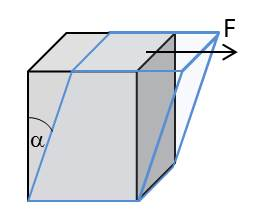
\includegraphics[width=.8\textwidth]{Abbildungen/Scherung.jpg}
	\captionof{figure}{Deformation eines Würfels durch Scherkräfte}
	\label{fig:Scherung}
\end{minipage}


\subsection{Beschreibung von Wellen}

Spannen wir ein Seil zwischen zwei Punkten fest ein und schlagen nahe eines der Enden (am Ort $x_0$) kurz darauf, so entsteht eine Auslenkung, die über die ganze Länge des Seils bis zum anderen Ende läuft, dort reflektiert wird und zurückläuft. So kann die Auslenkung mehrmals über das Seil hin- und herlaufen, ohne ihre Form stark zu ändern. Diese Form von Seilwellen kennen Sie aus dem Alltag von der Schwingung einer Saite oder, in zwei Dimensionen, als Ausbreitung einer Oberflächenwelle in Wasser.\\
Wir bezeichnen die Auslenkung $y$ des Seils am Ort $x$ und zur Zeit $t$ mit $y=f(x,t)$. Die ursprüngliche Auslenkung $f(x_0, 0)$ soll nach der Zeit $t$ um die Strecke $ct$ gewandert sein, $c$ bezeichnet also die Ausbreitungsgeschwindigkeit der Welle.\\
Ein undehnbares Seil können wir nur senkrecht zu seiner Richtung auslenken und so eine \textit{Transversalwelle} erzeugen. Bei einem dehnbaren Seil, oder äquivalent einer Schraubenfeder, können wir auch eine Auslenkung entlang der Richtung des Seils erzeugen, die sich dann als \textit{Longitudinalwelle} fortpflanzt.\\

\noindent
Betrachten wir einen Punkt auf dem Seil als Funktion der Zeit, so führt dieser eine Schwingung um die Ruhelage aus, wie wir sie in Versuch \ref{vn:1} kennengelernt haben. Wie wir wissen kommt eine Schwingung zustande, wenn es eine der Auslenkung proportionale Rückstellkraft gibt, welche in Richtung der Ruhelage wirkt.\\
Mit der Zugspannung $\sigma$ und der Dichte des Mediums $\rho$ können wir eine Wellengleichung aufstellen
\begin{equation*}
	\frac{d^2 y}{dt^2} = c^2\frac{d^2 y}{dx^2}\quad \mathrm{mit}\quad c^2 = \frac{\sigma}{\rho}\; .
\end{equation*}

\subsubsection{Schallgeschwindigkeit in Medien}

Eine ähnliche Wellengleichung kann man auch für den Fall elastischer Wellen in Festkörpern oder Flüssigkeiten aufstellen. Diese stellen wir als zeitlich und räumlich periodische Änderungen des Drucks des Mediums dar:
\begin{equation*}
	\ddot{p} = \frac{1}{\kappa\rho} p''\; ,
\end{equation*}
mit der Dichte $\rho$ des Mediums. Ist das Medium ein Festkörper ersetzen wir die Kompressibilität durch den Kehrwert des Elastizitätsmoduls und finden für die Geschwindigkeit dieser longitudinalen Schallwelle:
\begin{equation}
	c_{long} = \sqrt{\frac{1}{\kappa\rho}} = \sqrt{\frac{E}{\rho}}\; .
\end{equation}

In Elektrolyten kommt es mit zunehmender Konzentration zu einer Verringerung der Kompressibilität und zu einer Erhöhung der Dichte. Dies führt zu einer konzentrationsabhängigen Änderung der Schallgeschwindigkeit.

\subsubsection{Transversale Schallwellen}

Trifft eine longitudinale Schallwelle auf die Oberfläche eines Festkörpers und wird in diesen hinein transmittiert, so regt sie (vereinfachend dargestellt) die Atome des Festkörpers zu einer Schwingung entlang der Ausbreitungsrichtung der Welle und damit senkrecht zur Oberfläche des Festkörpers an. Diese Atome sind elastisch mit ihren Nachbarn gekoppelt, so dass diese ebenfalls zu Schwingungen angeregt werden. Betrachten wir diesen Vorgang als eine Verschiebung von Schichten des Festkörpers, die senkrecht zur Oberfläche stehen, so kann man aus diesen einen Quader zusammensetzen, der als ganzes durch die einlaufende Schallwelle in Form einer Scherung deformiert wird. \\
Es entsteht eine Welle, bei der die Atome senkrecht zur Bewegungsrichtung schwingen, also eine Transversalwelle. Mit den obigen Überlegungen überrascht es nicht, dass die Schallgeschwindigkeit dieser Transversalwelle durch das Schermodul bestimmt wird, anstelle des Elastizitätsmoduls, wie bei Longitudinalwellen:
\begin{equation}
	c_{trans} = \sqrt{\frac{G}{\rho}}\; .
\end{equation}
In Festkörpern, und nur in diesen, können sich also transversale Schallwellen ausbreiten, die Geschwindigkeit nicht gleich der Geschwindigkeit von Longitudinalwellen sind. Tabelle \ref{tab:Schallgeschwindigkeiten} zeigt einige Beispielwerte.

\begin{table}[hb]
	\centering
		\begin{tabular}{l|l|l}
			Material & $c_{long}$/ms$^{-1}$ & $c_{trans}$/ms$^{-1}$ \\
			\hline
			Aluminium & 6420 & 3020\\
			Blei & 1960 & 690\\
			Flintglas & 3980 & 2380\\
			Polyacryl & 2610 & 1430\\
		\end{tabular}
	\caption{Schallgeschwindigkeiten für longitudinale und transversale Wellenausbreitung in verschiedenen Festkörpern bei 20\degree~C.}
	\label{tab:Schallgeschwindigkeiten}
\end{table}

Wie man sieht, ist die Geschwindigkeit der longitudinalen Wellen immer größer als die der transversalen. Aus diesem Grund werden in der Seismologie longitudinale Erdbebenwellen, oder \textit{Kompressionswellen}, als Primär- oder P-Wellen bezeichnet. Entsprechend gilt für transversale Wellen, oder \textit{Scherwellen}, die Bezeichnung Sekundär- oder S-Wellen.\\

\noindent
Mit Hilfe einer etwas komplizierten Rechnung, die wir hier nicht vormachen wollen, kann man zeigen, dass die Amplitude der transmittierten Transversalwelle maximal wird, wenn sie sich im Festkörper unter einem Winkel von etwa 45\degree zur Oberflächennormalen ausbreitet. Im wohlbekannten Bild der Brechung einer Welle an einer Oberfläche (s. Versuch \ref{v:9}) ist das der Ausfallswinkel nach der Brechung. Nach dem Snellius'schen Brechungsgesetz gilt dann für den Einfallswinkel $\alpha$
\begin{equation}
	\frac{c_{trans}}{c_0} = \frac{\sin 45\degree}{\sin \alpha}\; ,
\end{equation}
wobei $c_0$ die Schallgeschwindigkeit in der umgebenden Flüssigkeit sei.\\
Damit wird der Einfallswinkel, unter dem die Amplitude der Transversalwelle maximal ist
\begin{equation}
	\sin \alpha_{max} = \frac{c_0}{c_{trans}} \sin 45\degree = \frac{c_0}{\sqrt{2}c_{trans}}\; .
\end{equation}
Wie bei der Brechung von Licht, kann der Ausfallswinkel $\beta = 90\degree$ werden, was der Totalreflektion der Transversalwelle entspricht. Für den Einfallswinkel gilt dann
\begin{equation}
	\sin \alpha_{tot} = \frac{c_0}{c_{trans}} \sin 90\degree = \frac{c_0}{c_{trans}}\; .
\end{equation}

\subsection{Erzeugung und Empfang von Ultraschall}

Bestimmte kristalline Stoffe sind in der Lage, einen mechanischen Druck in eine elektrische Spannung und umgekehrt eine elektrische Spannung in eine mechanische Deformation umzuwandeln. Diese Fähigkeit nennt man Piezoelektrizität.\\

\noindent
Ein Ultraschallwandler besteht aus einer Scheibe aus piezoelektrischem Material, deren Stirnflächen mit einer elektrisch leitfähigen Schicht überzogen sind. Legt man an die Stirnflächen eine elektrische Spannung, so entsteht zwischen ihnen ein elektrisches Feld. Das elektrische Feld übt eine Kraft auf die Gitterbausteine aus. Aufgrund vorhandener Unsymmetrien des aus positiven und negativen Ionen aufgebauten Gitters wirkt sich die Polarität des äußeren Feldes entweder verstärkend oder schwächend auf die Bindungskräfte innerhalb des Kristalls aus. Eine Verstärkung bedingt ein Zusammenziehen (Kontraktion), während eine Schwächung eine Ausdehnung (Dilatation) des Kristalls zu Folge hat. Die Frequenz, mit der die Scheibe kontrahiert und dilatiert, wird durch die angelegte Wechselspannung festgelegt.\\

\noindent
Der Piezokristall ist ein Oszillator, der durch die elektrische Wechselspannung zu erzwungenen Schwingungen angeregt wird. Dadurch hat er naturgemäß eine bestimmte Resonanzfrequenz, in welcher die Schwingungsamplitude und damit die abgestrahlte Intensität maximal sind. Die Resonanz hängt ab vom Material und den Dimensionen des Sender-Kristalls. Aus diesem Grund ist es notwendig, für jede gewünschte Ultraschallfrequenz einen speziell für diesen Zweck konstruierten Wandler zur Verfügung zu haben. Der Piezoeffekt ist umkehrbar. Derselbe Kristall kann daher sowohl als Sender, wie oben beschrieben, als auch als Empfänger genutzt werden. Die auf den Schallkopf auftreffenden Schallwellen, bzw. die Druckschwankungen am Ort des Schallkopfes, regen diesen zu mechanischen Schwingungen an, die sich an den Stirnflächen des Kristalls als elektrische Wechselspannung registrieren lassen.

\subsection{Anwendung: Sonographie}

Innerhalb der letzten 30 Jahre hat sich die Sonographie zu einer sehr wirkungsvollen Methode im Bereich der nichtinvasiven Diagnostik entwickelt. Man denke hier nur an die Schwangerschafts-Vorsorge oder die Funktionsdiagnostik in der Kardiologie. Das einfachste und zugleich älteste Verfahren ist das dem Echolot-Prinzip folgende A-Bild (A-Scan). Das A-Bild-Verfahren findet Anwendung in der Untersuchung des Auges, z.B. auf das Vorliegen einer Netzhautablösung und ist darüber hinaus die Grundlage aller anderen Ultraschall-Techniken.\\

\noindent
Im Folgenden soll das Grundprinzip des A-Bild-Verfahrens beschrieben werden: Der Schallsender gibt kurze Schallimpulse ab. Nach jedem Impuls wird der Sender abgeschaltet und arbeitet bis zum nächsten Impuls als Empfänger. Trifft der Impuls auf ein Objekt oder eine Grenzfläche, wird er dort ganz oder teilweise reflektiert.\\
Der reflektierte Impuls erreicht nach einer Zeit, die der doppelten Laufzeit (Hin- und Rückweg) zwischen dem Objekt und dem Schallkopf entspricht, den Empfänger und löst dort ein elektrisches Signal aus. Dessen Amplitude ist proportional zur Intensität des zurückgelangten Signals.\\
Man trägt nun in einem Diagramm die Stärke (Amplitude) des Echosignals über der Zeit auf, die seit dem Aussenden des Pulses vergangen ist. Diese Darstellung wird als A-Bild (Amplitude-Bild) bezeichnet. Für jeden neuen Sendepuls beginnt das Bild wieder neu (synchronisiert). Das dargestellte Zeitfenster wird so eingestellt, dass die reflektierten Signale aus den tiefsten darzustellenden Schichten innerhalb dieser Zeit am Empfänger eintreffen. Für den zeitlichen Abstand zwischen den Sender-Impulsen gilt darüber hinaus, dass er länger sein muss als die maximale Laufzeit eines Reflex-Signals. Jedes detektierte Echosignal erzeugt also im Empfänger eine elektrische Spannung, die nun verstärkt in $y$-Richtung über der Zeit ($x$-Achse) dargestellt wird. Die elektrische Verstärkung kann für längere Laufzeiten vergrößert werden, um die Verluste auf den längeren Laufwegen annähernd gleichmäßig zu kompensieren.\\

\noindent
Aus der Laufzeit $\Delta t$ des Reflex-Signals lässt sich über die Beziehung
\begin{equation*}
	\Delta s = c\cdot \Delta t
\end{equation*}
der doppelte Laufweg $\Delta s$ des Signals bestimmen.\\
Die Schallgeschwindigkeiten der verschiedenen Gewebearten (außer Knochen) sind annähernd gleich. Dies erlaubt es, die $x-$Achse mit einer Skala zu versehen, auf der jeder $x-$Wert einer bestimmten Tiefe des durchstrahlten Objektes entspricht. Aus dem Abstand zweier $y-$Auslenkungen ist dann direkt der Abstand der Schichten abzulesen, an denen der Schallimpuls reflektiert wurde.\\

\noindent
Eine übliche Erweiterung der Darstellungsform ist die Auftragung der reflektierten Amplitude als Helligkeit (Grauwert). Dadurch reduziert sich das Zeit-Amplituden-Diagramm ($x-y$-Diagramm, A-Scan) auf eine Linie mit verschieden hellen Punkten. Man kann nun viele solche Linien nebeneinander auftragen und erhält ein zweidimensionales Grauwertebild. In der Regel wird dabei die Eindringtiefe (bzw. Zeitachse) von oben vertikal nach unten angezeigt. Bildet man zeitlich aufeinander folgende A-Scans derart von links nach rechts ab, erhält man den sog. TM-Scan
(time mode).\\
Eine wichtige Anwendung des TM-Scans ist das Herzecho. Man schaut hier auf die Wanddicke des Herzens und deren Veränderung während des Schlagens. Daran lassen sich z.B. Klappenfehler und Herzinsuffizienzen erkennen.\\

\noindent
Um auch in Querrichtung Informationen zu erhalten, lässt man den Schallkopf nicht nur einmal den Schall aussenden und wieder einfangen, sondern scannt in verschiedenen Winkeln die Körperstrukturen ab. Die aneinandergesetzten A-Scan-Linien entsprechen nun verschiedenen Durchstrahlrichtungen und das Bild zeigt eine Schnittebene durch den Körper. Diese Darstellung heißt B-Bild oder B-Scan (von
brightness).

\begin{tutorhint}
%------------------------------------------------
\section{Fragen zur Vorbereitung}
%------------------------------------------------

\begin{enumerate} 
	\item Welche Deformation eines Festkörpers wird durch das Elastizitätsmodul beschrieben? Welche durch das Schubmodul? Geben Sie an, in welche Richtung jeweils die Kraft wirkt.
	%
	\item Wie groß ist die Schallgeschwindigkeit in Luft ungefähr?
	%
	\item Wieso treten transversale Schallwellen ausschließlich in Festkörpern auf und nicht in Fluiden?
	%
	\item Wie funktioniert die Ultraschall-Sonographie oder Echographie? Welche Größen werden gemessen?
	%
	\item Von welchen Größen hängt die Schallgeschwindigkeit in einem Fluid ab?
	%
	\item Wie funktioniert die Konzentrationsmessung in einem Elektrolyten per Ultraschall? 
\end{enumerate} 
\end{tutorhint}

%------------------------------------------------
\section{Durchführung} 
%------------------------------------------------

\subsection{Vorbereitung}

Schließen Sie die beiden Ultraschallsonden an den \verb RECEIVER  bzw. \verb TRANSMITTER -Ausgang des Betriebsgeräts an.
Auf dem PC als Benutzer \verb prakt  einloggen (kein Passwort), das Betriebsgerät anschalten und auf dem PC das Programm \verb AScan  starten. Im oberen Teil der Anzeige ist der Zeitverlauf der Amplitude des empfangenen Signals zu sehen, im unteren der Zeitverlauf der Verstärkung. Unter \verb RECEIVER  kann zwischen \verb REFLECT.  und \verb TRANS. , also reflektiertem bzw. transmittiertem Signal an Hand der Laufzeit unterschieden werden. Auf transmittiertes Signal stellen. \\
In der Menüleiste des Programms auf die volle Zeitachse stellen (der Knopf neben Stop sollte \verb Half  anzeigen, ansonsten \verb Full  drücken). Eine Bedienungsanleitung des Steuergeräts befindet sich auf dem Desktop unter dem Icon \verb AScan  Handbuch.
\begin{figure}[h!]
	\begin{center}
		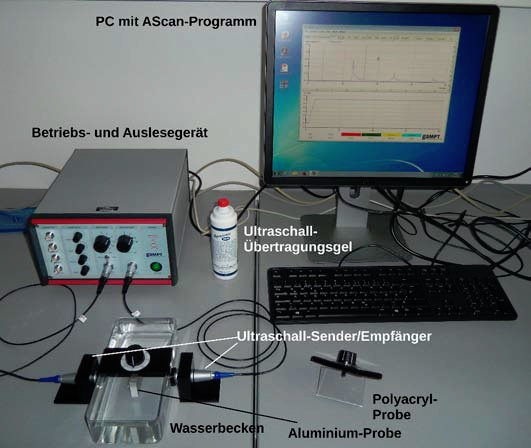
\includegraphics[width=0.90\textwidth]{Abbildungen/Ultraschall_Aufbau.jpg}
	\end{center}
\end{figure}

\begin{hint}
	Ab und zu kommt es zu Störungen in der USB-Verbindung zwischen dem PC und dem Ultraschall-Betriebsgerät. In dem Fall führt zum Beispiel eine Erhöhung der Sendeleistung oder der Verstärkung des Empfängers NICHT zu einer höheren Amplitude des am PC dargestellten Signals.\\
	Beenden Sie das Programm \verb AScan und schalten Sie das Betriebsgerät aus. Ziehen Sie den USB-Stecker raus und stecken ihn nach ein paar Sekunden wieder ein. Wenn Sie jetzt \verb AScan wieder starten, sollte die Kommunikation wieder funktionieren.
\end{hint}

\subsection{Durchführung}

\begin{enumerate}
	%%%%%%%%%%%%%%%%%%%%%%%%%%%%%%%%%%%%%%%%%%%%%%%%%%%%%%%%%%%%%%%%%%%%%%%%%%%%%%%%%%%%%%%%%%%%%%%%%%%%
	% Teil 1
	%%%%%%%%%%%%%%%%%%%%%%%%%%%%%%%%%%%%%%%%%%%%%%%%%%%%%%%%%%%%%%%%%%%%%%%%%%%%%%%%%%%%%%%%%%%%%%%%%%%%
	\item \textbf{Schallgeschwindigkeit als Funktion der Temperatur}
	\begin{enumerate}
		\item Füllen Sie die große Wanne zu etwa einem Drittel mit Leitungswasser und fügen Sie Eis hinzu. Mischen Sie so lange, bis das Wasser eine Temperatur von 0\degree C hat und keine Eiskristalle mehr darin schwimmen. \textbf{Das ist sehr wichtig, da diese die Pumpe des Durchlauferhitzers beschädigen können.}
		%
		\item Platzieren Sie den Ultraschallsender und -empfänger so, dass eine unbehinderte Sichtlinie zwischen den beiden besteht. Vergessen Sie nicht, das Ultraschall-Übertragungsgel zu verwenden.\\
		Stellen Sie die Verstärkung am Betriebsgerät unter \verb RECEIVER  auf den kleinsten Wert und stellen Sie die Ausgangsleistung unter \verb TRANSMITTER  so ein, dass das empfangene Signal gut erkennbar ist und unter 1,2V liegt, da ansonsten der Verstärker in Sättigung geht.
		%
		\item Messen Sie den Abstand zwischen den beiden Sonden.
		%
		\item Messen Sie die Laufzeit des Ultraschallpulses bei etwa 0\degree C mit Hilfe des ersten Cursors. Wie genau ist die Zeitmessung?
	\end{enumerate}
	%
	Für die nun folgende Messung der Schallgeschwindigkeit als Funktion der Temperatur empfiehlt es sich, das ein Praktikant den PC bedient und der/die andere die Temperatur im Auge behält und die Messwerte notiert. Zur Messung der Änderung der Laufzeit des Ultraschallpulses empfiehlt es sich, den ersten Cursor bei der ursprünglichen Laufzeit zu lassen und mit dem zweiten Cursor die neue Laufzeit zu messen. Das Programm berechnet automatisch die Differenz der beiden Zeiten in $\mu$s.
	%
	\begin{enumerate} \setcounter{enumii}{3}
		%
		\item Starten Sie den Lauda Durchlauferhitzer. Stellen Sie die Solltemperatur auf 35\degree~C. Der Durchlauferhitzer fängt sofort an, das Wasser aufzuheizen, behalten Sie daher die Anzeige der Isttemperatur im Auge.
		%
		\item Messen Sie die Laufzeitdifferenz des Ultraschallpulses als Funktion der Temperatur in Schritten von etwa 2\degree~C. Schätzen Sie die Unsicherheit der Temperaturmessung ab.
	\end{enumerate}
	%
	%%%%%%%%%%%%%%%%%%%%%%%%%%%%%%%%%%%%%%%%%%%%%%%%%%%%%%%%%%%%%%%%%%%%%%%%%%%%%%%%%%%%%%%%%%%%%%%%%%%%
	% Teil 2
	%%%%%%%%%%%%%%%%%%%%%%%%%%%%%%%%%%%%%%%%%%%%%%%%%%%%%%%%%%%%%%%%%%%%%%%%%%%%%%%%%%%%%%%%%%%%%%%%%%%%
	\item \textbf{Schallgeschwindigkeit als Funktion der Salzkonzentration}
	\begin{enumerate}
		\item Füllen Sie die kleine Wanne mit Leitungswasser, so dass die beiden an der Längsseite außen angebrachten Sonden vollständig bedeckt sind (für die Anbringung das Ultraschall-Übertragungsgel verwenden). Benutzen Sie hierfür den Messbecher und notieren Sie das Volumen des Wassers, da Sie dieses zur Berechnung der Salzkonzentration brauchen.
		%
		\item Messen Sie die Laufzeit des Ultraschallpulses in Leitungswasser mit dem 1. Cursor.
		%
		\item Stellen Sie nun mit dem Kochsalz Lösungen von 25, 50, 75, 100, 150, 200, 250~g/l her und messen Sie jeweils die Laufzeitdifferenz des Ultraschallpulses mit Hilfe des zweiten Cursors. Bevor Sie die  Messung durchführen können müssen die Salzkristalle komplett gelöst sein. Wieso ist das so?\\ 
		Schätzen Sie die Unsicherheit der Kochsalzkonzentration Ihrer Lösung ab.
		%
		\item Bitte waschen Sie die Schale mit der Salzlösung nach Ende des Versuchs ordentlich unter fließendem Wasser aus. Ansonsten bilden die Rückstände Salzblumen, die zwar schön anzusehen sind, aber die Messungen der nächsten VersuchsteilnehmerInnen verfälschen.
	\end{enumerate}
	%%%%%%%%%%%%%%%%%%%%%%%%%%%%%%%%%%%%%%%%%%%%%%%%%%%%%%%%%%%%%%%%%%%%%%%%%%%%%%%
	% Teil 3: Alternativ für Geowissenschaftler
	%%%%%%%%%%%%%%%%%%%%%%%%%%%%%%%%%%%%%%%%%%%%%%%%%%%%%%%%%%%%%%%%%%%%%%%%%%%%%%%
	\item \textbf{Für Geowissenschaftler an Stelle von Versuchsteil 2: \\
		Longitudinale und transversale Schallwellen in Festkörpern}
	\begin{enumerate}
		\item Platzieren Sie die Polyacrylplatte in die Mitte des Beckens und stellen Sie mit dem Knopf den Winkel der Platte auf 20\degree .\\
		Es sollte nun zwei Signale, ggf. mit einem ''Satelliten'' zu sehen sein (durch Mehrfachreflexion, diese ignorieren): das frühere Signal entspricht wegen der etwa zweifach größeren Schallgeschwindigkeit der longitudinalen Schallwelle, das spätere entsprechend der transversalen Welle. Messen Sie die Amplitude beider Signale mit dem hellblauen Cursor im \verb AScan -Programm als Funktion des Auftreffwinkels in Schritten von 5\degree~zwischen 0\degree~und 90\degree; ggf. während der Messung die Verstärkung erhöhen.
		%
		\item Wiederholen Sie diese Messung analog mit der Aluminiumplatte.
	\end{enumerate}
	%
\end{enumerate}


%------------------------------------------------
\section{Auswertung} 
%------------------------------------------------
\etodo{Musterauswertung}

\begin{hint}
	Bitte fertigen Sie die Graphen in der folgenden Auswertung per Hand auf Millimeterpapier an.
\end{hint}

\begin{enumerate}
	%%%%%%%%%%%%%%%%%%%%%%%%%%%%%%%%%%%%%%%%%%%%%%%%%%%%%%%%%%%%%%%%%%%%%%%%%%%%%%%%%%%%%%%%%%%%%%%%%%%%
	% Teil 1
	%%%%%%%%%%%%%%%%%%%%%%%%%%%%%%%%%%%%%%%%%%%%%%%%%%%%%%%%%%%%%%%%%%%%%%%%%%%%%%%%%%%%%%%%%%%%%%%%%%%%
	\item\textbf{Schallgeschwindigkeit als Funktion der Temperatur}
	\begin{enumerate}
		\item Berechnen und tabellieren Sie die Laufzeiten der Ultraschallpulse als Funktion der Temperatur aus dem Wert bei 0\degree~C und den gemessenen Laufzeitunterschieden.
		%
		\item Berechnen Sie aus dem gemessenen Abstand zwischen Ultraschallsender und -empfänger, sowie aus den Laufzeiten der Pulse die Schallgeschwindigkeit in Wasser als Funktion der Temperatur. Wie groß ist die Unsicherheit der Werte?
		%
		\item Tragen Sie die berechneten Schallgeschwindigkeiten gegen die Temperatur auf. Beachten Sie, dass sowohl die Schallgeschwindigkeit, wie auch die Temperatur bei der sie gemessen wurde Unsicherheiten haben.
		%
		\item Die Schallgeschwindigkeit in Leitungswasser sollte bei Raumtemperatur $c=1480$~m/s betragen. Stimmt diese Angabe mit Ihren Messwerten überein? Wenn nicht, warum nicht?
	\end{enumerate}
	%
	%%%%%%%%%%%%%%%%%%%%%%%%%%%%%%%%%%%%%%%%%%%%%%%%%%%%%%%%%%%%%%%%%%%%%%%%%%%%%%%%%%%%%%%%%%%%%%%%%%%%
	% Teil 2
	%%%%%%%%%%%%%%%%%%%%%%%%%%%%%%%%%%%%%%%%%%%%%%%%%%%%%%%%%%%%%%%%%%%%%%%%%%%%%%%%%%%%%%%%%%%%%%%%%%%%
	\item \textbf{Schallgeschwindigkeit als Funktion der Salzkonzentration}
	\begin{enumerate}
		\item Die Schallgeschwindigkeit in Leitungswasser beträgt bei Raumtemperatur \\
		$c~=~1480$~m/s. Für die Schallgeschwindigkeit bei einer gegebenen Salzkonzentration $\tilde{c}$ gilt:
		\begin{equation}
			\tilde{c} = c\cdot\frac{t_0}{t_0-\Delta t}
		\end{equation}
		Berechnen und tabellieren Sie die Schallgeschwindigkeiten $\tilde{c}$ für die verschiedenen Salzkonzentrationen aus den gemessenen Laufzeitunterschieden. 
		%
		\item Tragen Sie die Schallgeschwindigkeit gegen die Konzentration der Salzlösung auf und und bestimmen Sie Steigung und Achsenabschnitt einer Ausgleichsgeraden inkl. ihrer Unsicherheiten. Beachten Sie, dass sowohl die Schallgeschwindigkeit als auch die Konzentration Unsicherheiten haben.
		%
		\item Der Achsenabschnitt der Ausgleichsgeraden gibt die Schallgeschwindigkeit bei einer Salzkonzentration von 0~g/l an. Stimmt der gemessene Wert mit der oben angegebenen Schallgeschwindigkeit in Leitungswasser überein? \\
		Wenn nicht, warum nicht?
	\end{enumerate}
	%
	%%%%%%%%%%%%%%%%%%%%%%%%%%%%%%%%%%%%%%%%%%%%%%%%%%%%%%%%%%%%%%%%%%%%%%%%%%%%%%%%%%%%%%%%%%%%%%%%%%%%
	% Teil 3
	%%%%%%%%%%%%%%%%%%%%%%%%%%%%%%%%%%%%%%%%%%%%%%%%%%%%%%%%%%%%%%%%%%%%%%%%%%%%%%%%%%%%%%%%%%%%%%%%%%%%
	\item \textbf{Schallgeschwindigkeit longitudinaler und transversaler Wellen}
	\begin{enumerate}
		\item Tragen Sie jeweils die Amplitude der longitudinalen und der transversalen Welle gegen den Winkel auf. Bestimmen Sie den Winkel des ersten Verschwindens der Welle. Dieser entspricht dem Winkel für Einsetzen der Totalreflexion. Berechnen Sie daraus die entsprechende longitudinale und transversale Schallgeschwindigkeit in beiden Festkörpern.
		%
		\item Bestimmen Sie das Maximum der Amplitude des transversalen Signals und berechnen Sie hieraus ebenfalls die transversale Schallgeschwindigkeit.
		%
		\item Vergleichen Sie beide Messergebnisse zur transversalen Schallgeschwindigkeit und beide Schallgeschwindigkeiten mit den entsprechenden Literaturwerten.
	\end{enumerate}
\end{enumerate}

\end{document}